


\documentclass[crop,tikz,border=0pt,12pt]{standalone}

\usepackage{amsthm,amsmath,latexsym,mathtools}


%Custom definitions
\newcommand{\avec}{\mathbf{a}}
\newcommand{\bvec}{\mathbf{b}}
\newcommand{\uvec}{\mathbf{u}}
\newcommand{\vvec}{\mathbf{v}}
\newcommand{\wvec}{\mathbf{w}}
\newcommand{\setN}{\mathbb{N}}
\newcommand{\setZ}{\mathbb{Z}}
\newcommand{\setQ}{\mathbb{Q}}
\newcommand{\setR}{\mathbb{R}}
\newcommand{\setC}{\mathbb{C}}
\newcommand{\setF}{\mathbb{F}}


\begin{document}

 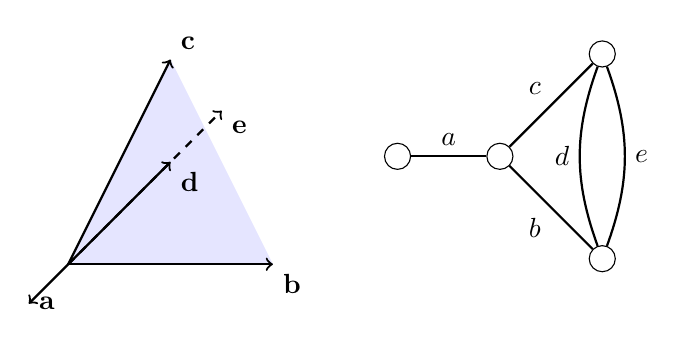
\begin{tikzpicture}[scale=1.3]
 \begin{scope}
   % Define the plane
  \fill[blue!10] (0,0,0) -- (2,0,0) -- (1,2,0) -- cycle;
  % Draw the vectors
  \draw[thick, ->] (0,0,0) -- (2,0,0) node[below right] {$\mathbf{b}$};
  \draw[thick, ->] (0,0,0) -- (1,2,0) node[above right] {$\mathbf{c}$};
  \draw[thick, ->] (0,0,0) -- (1,1,0) node[below right] {$\mathbf{d}$};
  \draw[thick, ->, dashed] (0,0,0) -- (1.5,1.5,0) node[below right] {$\mathbf{e}$};
  \draw[thick, ->] (0,0,0) -- (0,0,1) node[right] {$\mathbf{a}$};
\end{scope}
 \begin{scope}[xshift=120,yshift=30]
  % Define the vertices
  \node[circle, draw, fill=white] (1) at (0,0) {$$};
  \node[circle, draw, fill=white] (2) at (-1,0) {$$};
  \node[circle, draw, fill=white] (3) at (1,1) {$$};
  \node[circle, draw, fill=white] (4) at (1,-1) {$$};
  % Draw the edges
  \draw[thick] (1) -- (2) node[midway, above] {$a$};
  \draw[thick] (1) -- (4) node[midway, below left] {$b$};
  \draw[thick] (1) -- (3) node[midway, above left] {$c$};
  \draw[thick, bend right=20] (3) to node[midway, left] {$d$} (4);
  \draw[thick, bend left=20] (3) to node[midway, right] {$e$} (4);
  % Labeling positions
  \node at (0, 0.5) {}; % Adjust space if needed
\end{scope}
\end{tikzpicture}

\end{document}
